\documentclass[12pt,letterpaper]{article}

\usepackage{url}
%\usepackage{hyperref}
\usepackage{amsmath}
\usepackage{amsthm}
\usepackage{amssymb}
\usepackage{amsfonts}
\usepackage{pdfsync}
\usepackage [font=small, labelfont=bf]{caption}
\usepackage{color}
\usepackage{bm}
%\usepackage{natbib}
\usepackage{graphicx}

\theoremstyle{definition}
\newtheorem{dfn}{Definition}

\begin{document}

% The numbers below controls the amount of space between the following sections
\def\shiftdowna{0.32in}  % Adjust for balance
\def\shiftdownb{0.22in}  % Adjust for balance

% Set up the boiler plate at the top of the page

\begin{center}
\textbf{{\large Project Work Statement}}\\


% SPONSOR
\vspace \shiftdowna
\underline {Sponsor}\\ 
\vspace{5pt}
\textbf{{\large Blue Jays Unlimited}}\\


% TITLE
\vspace \shiftdowna
\textbf{{\large Modeling and Simulating Fan Participation at Large Scale Sporting Events}}


% STUDENTS
\vspace{0.35in}
\vspace \shiftdownb
\underline {Participants} \\
\vspace{5pt}
Ahmed Aly, \texttt{aaly2@jhu.edu}\\
\vspace{3pt}
Steven Su, \texttt{ssu7@jhu.edu}\\
\vspace{3pt}
Danni Tang, \texttt{dtang9@jhu.edu}

% SPONSORS
%\vspace \shiftdownb
%\underline {Potential Participants}\\
%\vspace{5pt}
%Youngser Park, \texttt{parky@jhu.edu} \\
%\vspace{3pt}
%\text{Mihn Tang}, \texttt{mtang10@jhu.edu} \\
%\vspace{3pt}
%\text{Glen Coppersmith}, \texttt{coppersmith@jhu.edu}

% DATE
\vspace \shiftdowna
Date: \today

\end{center}

\vfill  
%Fill page to force following note to bottom
\footnoterule
\noindent \small{Any apparent association of this work to Blue Jays Unlimited is
fictional one, and the sole purpose of this work is a class exercise.}

\newpage

\section{Background}

\paragraph{}
Blue Jays Unlimited (BJU), established in 1995, is a volunteer group of alumni, friends and staff dedicated to supporting and promoting Johns Hopkins athletics \cite{bjuwebsite}. BJU is the official booster club for Johns Hopkins athletics and has more than 3000 active members, who have raised more than \$4 million in funds to improve the Johns Hopkins athletic experience for both student athletes and fans alike \cite{bjuwebsite}. These funds provide money for capital projects as well as scholarship and operational endowments \cite{bjuwebsite}. BJU is present at nearly all major Johns Hopkins sporting events to encourage fans to support their Blue Jays in a vociferous and family-friendly manner to propel their Hopkins' teams to victory. It is their goal to provide Johns Hopkins' athletic teams with the ultimate advantage: a spirited home crowd. 

%GeoEye is a leading source of geospatial information and insight for decision
%makers and analysts who need a clear understanding of our changing world to
%protect lives, manage risk, and optimize resources. Each day, organizations in
%defense and intelligence, public safety, critical infrastructure, energy, and
%online media rely on GeoEye's imagery, tools, and expertise to support
%important missions around the globe. Widely recognized as a pioneer in
%high-resolution satellite imagery, GeoEye has evolved into a complete provider
%of geospatial intelligence solutions. GeoEye's ability to collect, process,
%and analyze massive amounts of geospatial data allows our customers to quickly
%see precise changes on the ground and anticipate where events may occur in the
%future.

\section{Problem Statement}

\paragraph{}
A loud and supportive home crowd is the ultimate home team advantage for any collegiate sports team. As such, maximizing fan participation in events such as chanting the school fight song, waving a rally towel, or doing the wave is greatly desired. These events will hence be collectively termed `cheering'.
\paragraph{}
BJU is interested in maximizing the amount of fan participation in cheering at sporting events held on Homewood Field at the Homewood campus of Johns Hopkins University in Baltimore, MD. More specifically, they believe that they can increase fan participaton in cheering events by strategically placing volunteer `cheer starters' in the home crowd to lead and urge other fans to participate in these cheering events.

\section{Objectives}
\paragraph{}
Our task is to provide BJU with a simple model as well as simulation results from the model which determine if their belief about cheer starters is accurate. Furthermore if this belief is true, we will try to provide BJU with more details about the quantity and location at which these cheer starters should be placed within the home crowd at Homewood Field in order to maximize fan participation.

\begin{figure}[h]
	\begin{center}
			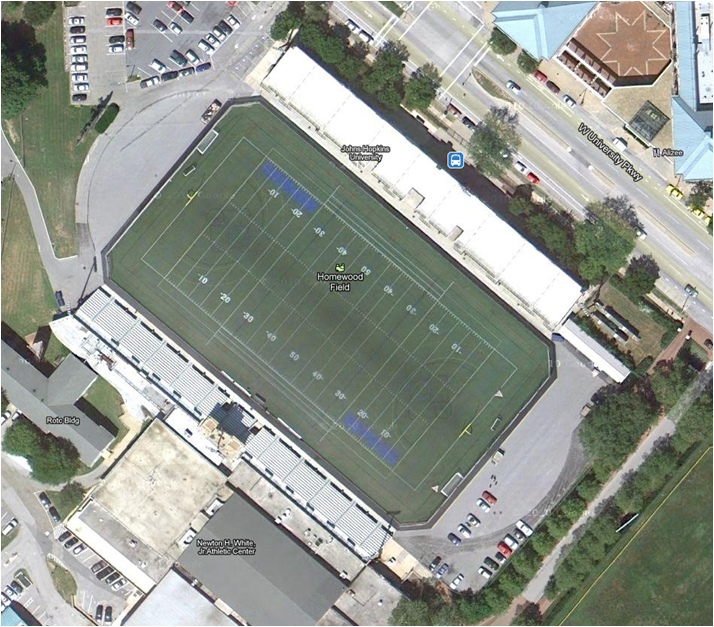
\includegraphics[height=3in] {HomewoodField.png}
	\end{center}
	\caption{Homewood Field located on the Homewood Campus of Johns Hopkins University in Baltimore, MD. The bleachers in the lower left corner are traditionally where the home team's fans sit.}
	\label{fig:homewoodfield}
\end{figure}

\paragraph{}
Consider the satelite image of Homewood Field in Figure \ref{fig:homewoodfield} courtesy of Google Maps. Homewood Field's capacity is approximately 8500 spectators \cite{wiki}. The long rectangular section of bleachers in the lower left of portion of the image seats approximately 4000 fans and is traditionally reserved for Blue Jays' fans. For nearly all major Hopkins' sporting events, these home team bleachers are filled to capacity. As such, BJU is specifically interested in maximizing the fan cheering in these home team bleachers. 

%\begin{figure}[h]
    %\begin{center}
        %\includegraphics[width=\textwidth]{../images/sholmesbike.png}
    %\end{center}
    %\caption{A bicycle track}
    %\label{fig:biketrack}
%\end{figure}

%To simplify our problem, we assume that the track is generated by a moving 
%bicycle.  It is easy to see that the bicycle is swerving left and right,
%but the general direction of the movement is not so obvious.  Nevertheless,
%one can also identify the direction of the bicycle. 

%The sponsor currently has a limited capability to make such inference from a
%track of moving object from an image, and our task is to provide them with 
%a reasonably large collection of such features and algorithms to detect them. 


\section{Approach}
\paragraph{}
We will develop a stochastic model which uses several parameters to determine whether a single fan will participate in cheering. These model parameters will account for the number of other fans seated around a given fan that are cheering as well as the given fan's innate level of support of the team. The more people surrounding a fan who are cheering and the greater the level of the fan's support of the team, the more likely the fan will join in the cheering. This model for a single fan will be stochastic in the sense that the support level for the team will be randomized between fans. This more accurately reflects reality where different fans can have different levels of support for the same team. 
\paragraph{}
By repeatedly employing this single fan model, we can simulate a large crowd of fans seated in a spatial arrangment similar to the home team bleachers at Homewood Field and create a multi-fan model. Due to computational limits, we will downscale Homewood Field and model a home crowd of between 100-1000 fans. We will run this multi-fan model successively for multiple cycles; each cycle will represent a new time point after the initial start of the cheering and will show how many more fans have begun cheering at that given time point. At the end of the cycles, we will calculate the total percentage of fans who have joined in the cheering. Using Monte Carlo methods we will repeatedly run this procedure to get an average percentage of fan participation for a given cheer starter setup. If time permits we can then repeat these Monte Carlo simulations for various cheer starter setups to determine if there are any patterns in setups which maximize fan participation. 
\paragraph{}
The model will be coded using MATLAB R2009b. Computations will be performed on a Intel Core i7 desktop PC. 

%Given a limited amount of our times, we will assume that extraction of 
%tracts from an image is already completed.   
\section{Milestones}
We have the following major deadlines:
\begin{itemize}
    \item Work Statement due date, Sep 28, 2012.
    \item Midterm Presentation due date, Oct 17, 2012.
    \item Progress Report due date, Oct 26, 2012.
    \item Final Presentation due date, Nov 16, 2012.
    \item Final Report due date, Nov 30, 2012.
\end{itemize}

\section{Deliverables}
\subsection{From Team to Sponsor} % (fold)
The following outputs are expected from this project:
\begin{itemize}
    \item MATLAB R2009b and R combination package which simulates cheering. The main simulation code will be written in MATLAB. All documentation for the MATLAB code will be done in R. We will also provide MATLAB scripts that can be used to reproduce our numerical and simulation test results. If we do not finish learning the necessary R documentation code in class by Novemeber 9, we will provide documentation in an appropriate alternative method.
    \item If time permits, a list of patterns of cheer starter setups (i.e.~number of cheer starters and location of them) that maximize fan cheering.
    \item Technical report and presentations summarizing the work. 
\end{itemize}

\subsection{From Sponsor to Team} % (fold)

In order for our project to be successful, we will need:
\begin{itemize}
    \item Timely responses to inquiries 
\end{itemize}


\newpage
%\begin{thebibliography} {1}

\bibliographystyle{plain}
%\renewcommand
%\bibname{Selected Bibliography Including Cited Works}
%\nocite{*}
\bibliography{biblioWS}
%\bibitem{bjuwebsite} http://www.hopkinssports.com/bluejays-unlimited/
%\bibitem{wiki} http://en.wikipedia.org/wiki/Homewood\_Field
%\bibliography{biblio}
%\end{thebibliography}

\end{document}
